\documentclass[12pt]{article}

\usepackage[utf8]{inputenc}
\usepackage{setspace}
\usepackage[
	a4paper,
	total={17cm,25cm},
	top=3cm, left=2cm,
	includefoot
	]{geometry}
\usepackage[
	english,
	czech
	]{babel}
% České citace
\usepackage[autostyle]{csquotes}
\usepackage{caption}
% Grafika a obrázky
\usepackage{graphicx}
\graphicspath{{./assets/}}
% Odsazení pro odstavce
\setlength{\parskip}{5pt}

\title{Správa Office 365}
\author{Petr Maronek}
\date{5.12.2022}

% 	Vysvětlivky
%	\section* hvězdička znamená, že má LaTeX odebrat číslování

\begin{document}
    \begin{sloppypar}
	\begin{spacing}{1.15}
        % Odstrnění  číslování pro titulní list (a reset na 1)
        \pagenumbering{gobble}
        \rmfamily
		\maketitle
		\begin{center}
			\textbf{Vysoká škola finanční a správní}\linebreak
			Projektování Informačních Systémů 1\linebreak
			Zimní semestr 2022\linebreak
			Vedoucí práce: \textbf{Ing. Václav Řezníček, Ph.D.}
		\end{center}
		\pagebreak
        % Arabské číslování stránek (a reset na 1)
		\pagenumbering{arabic}

		\section*{Abstrakt}
		Správa Officu 365, konkrétně SharePointu Online a Microsoft Teams, je pro velké 
        firmy čím dál náročnější. Má aplikace, kterou tato práce popisuje a implementuje, 
        se tuto problematiku pokouší přímo vyřešit a celou správu tak učinit přístupnější 
        pro administraci a případnou rozšiřitelnost. Spolu s modelem správy, který musí 
        zajistit korporátní zásady pro uchování dat, je také zásadní implementace v cloudovém 
        prostředí Microsoft Azure. Celý model zohledňuje požadavky na retenci dat, bezpečnost 
        z hlediska přístupů a datové hygieny.

		\section*{Klíčová slova}
		Office365, Microsoft, proces, automatizace, korporace, cloud
		\pagebreak
		    
		\section*{Úvod}
	    Office 365 je rozsáhlý ekosystém byznysových aplikací, které pracovníkům
        v mnoha ohledech usnadňují každodenní pracovní povinnosti. Jedná se o 
        nejrozšířenější kancelářský software na světě a mnoho velkých 
        nadnárodních korporací jej používá v mnoha aspektech své činnosti. 
        Tato činnost však může být svázána místními předpisy nebo regulací 
        podnikání v určité oblasti, jako například farmacie, energetika nebo 
        potravinářství. Z této podstaty ovšem vyplývá, že se tento software musí
        řídit zásadami a politikami jednotlivých firem, aby splňoval různá 
        omezení nebo dokonce blokovat některé ze svých funkcí. V této práci se 
        zaměřím hlavně na SharePoint Online a Microsoft Teams, které jsou v celém 
        ekosystému Office 365 nejvíce používané, zejména jako úložiště dokumentů 
        a centrum sdílení napříč jednotlivými divizemi firmy. Právě životní 
        cyklus dokumentů je základní linií v každé firemní politice, která 
        podléhá místním regulím nebo externím auditům. Pro účely textu
        budu aplikace SharePoint Online a MS Teams souhrnně nazývat jako
        \textit{pracovní prostory} nebo čistě \textit{prostory}. 

        Jak nejlépe poskytnout uživatelům přístup k těmto technologiím a zároveň 
        zajistit shodu s firemními a státními předpisy? Také nemůžeme spoléhat na 
        uživatele, že budou aktivně dodržovat všechna pravidla a nařízení, která 
        dané úložiště musí splňovat. V neposlední řadě musí být celé řešení do 
        jisté míry automatizované, aby administrátorský tým Office 365 nebyl 
        zavalen desítkami až stovkami požadavků denně na vytvoření SharePointu 
        nebo Teams.
        
        Hlavními ukazateli výsledku této práce budou především doba splnění 
        uživatelských požadavků, celková úspora času v "man-days" administrátorského 
        týmu a úspora z hlediska financí. Budu také předpokládat, že má dostatek
        financí a času na implementaci požadovaných změn z hlediska nasazení řešení
        pomocí cloudových služeb. A také, že má i prostor vyjednávat o ceně dodávaného
        software jelikož se jedná pro dodavatele o velkého zákazníka. Pro
        zjištění současného stavu využiji analýzy SWOT, která se pro potřeby
        této práce hodí nejlépe.
        
        \section*{Současný stav}
        V této sekci projdu celé stávající řešení, jeho výhody a naopak nevýhody
        z hlediska nákladů na provoz, administrace a uživatelské přístupnosti.
        Nejprve nastíním pohled na celý systém a čemu slouží a poté provedu SWOT
        analýzu, podle které identifikuji potencionální slabiny a možnosti ke
        zlepšení.

        Modelová forma pro tuto práci podniká v oblasti farmacie. Má rozsáhlý
        systém přidělování licencí a vytváření pracovních prostorů, který však
        trpí zejména na dlouhé čekací lhůty ze strany technologie, která
        nedokáže díky složitým schvalovacím procesům tyto prostory vytvořit v
        rámci hodin. Nejkritičtější části tohoto procesu stále vyžadují manuální
        intervenci ze strany administrátorského týmu, což v konečném důsledku
        znamená frustraci ze strany uživatelů, kteří tyto pracovní prostory
        vyžadují relativně rychle. Současný proces je schopný uspokojit žádost
        uživatele o nový prostor v průměru za 24 hodin. Tato hodnota je však v
        dnešní době, kdy jsou možnosti automatizace procesů  informačních 
        technologií na vysoké úrovni, pro mnoho uživatelů neakceptovatelná a
        a proces si tedy žádá revizi. 
        
        Systém má za primární úkol poskytnout uživatelům jednoduchou správu nad
        svými virtuálními prostory v rámci Office 365. Systém ve svém rámci řídí 
        důležité procesy, které jsou v souladu s certifikacemi informačních 
        technologií a navíc splňuje politiky nastavené svou společností. Procesy 
        v systému jsou například vytvoření pracovního prostoru, smazání pracovního 
        prostoru, automatické notifikace o expiraci pracovních prostorů nebo chybějících 
        metadatech a nebo zažádání o speciální funkce v rámci těchto prostorů. Systém také
        automaticky nastavuje spoustu vlastností pro tyto prostory jako jsou
        přístupová práva, firemní branding nebo nasazení povinných firemních
        aplikací. Je tedy zřejmé, že systém není vytvořen pouze pro uživatele,
        ale také zajišťuje shodu s firemními politikami.

        Z technického hlediska je v současnosti celý systém nasazen v cloudovém 
        prostředí poskytovaném Microsoftem Azure. Nicméně celé řešení je stále 
        koncipováno do podoby, jak bylo původně vytvořené pro hostování na 
        vlastních serverech spolu s technologiemi té doby. Celé řešení je v 
        současné době již přes 5 let staré a i když stále funguje podle firemních 
        požadavků, může v blízké budoucnosti dojít k jeho častým poruchám. To by
        znamenalo pro firmu v krajním případě i nemalé ztráty. A právě proto se 
        nyní pokusím zjistit, jak tomuto scénáři předejít a navíc celý proces
        vylepšit.

        \subsection*{SWOT Analýza}
        Nejprve se zaměřím na \textbf{silné stránky} současného řešení. Protože
        je systém z části poskytovaný softwarovým dodavatelem třetí strany
        (hlavně z důvodu uživatelského rozhraní), je z podstaty velice stabilní a
        dostupnost se pohybuje v horních 99\%. Díky tomu mají uživatelé důvěru v
        systém samotný a zbytečně negenerují emaily směrem k podpoře. Pro
        uživatele je zde také samotné prostředí, ve kterém se pohybují.
        Microsoft sice poskytuje grafické prostředí pro vytváření zmíněných
        prostorů, nicméně se jedná o prostředí, které není příliš intuitivní a 
        z administrátorského hlediska příliš strohé na jakoukoliv
        rozšiřitelnost. Proto se firma před pěti lety rozhodla využít software
        třetí strany, aby poskytla uživatelům portál pro všechny své požadavky.
        Další silnou stránkou jsou nízké nároky na správu a to je zejména pro 
        administrátory velkou devízou. Tím, že se nemusí stále starat o chod
        systému, mohou svou práci přesunout jinam, kde jsou více potřeba. Systém
        stále vyžaduje jistou úroveň administrace, je nicméně znatelně ponížená
        oproti jiným řešením. Neposledním pozitivem současného řešení je také
        softwarová podpora, která je poskytována právě dodavatelskou
        společností. Ochota a rychlost řešení problémů je v tomto případě
        vitální a proto ji zařazuji mezi silné stránky.

        Ke \textbf{slabým stránkám} primárně patří formát dodávky softwaru. Není
        totiž vůbec jednoduché
        ho jakkoliv přizpůsobit požadavkům ať už administrátorů, tak firmy. Celý
        software je dodáván "AS-IS" a poskytuje minimální možnosti dodatečné
        konfigurace. To vede k již výše zmíněným prodlevám ve vytváření
        prostorů, kde je nutné požadavky manuálně schvalovat. V tomto ohledu je
        manuální vstup do procesu zásadním nedostatkem, protože je firma
        globální a požadavky přicházejí takřka v průběhu celého dne. Navíc, celý 
        tým administrátorů pracuje pouze ve východo-americké časové zóně a tudíž
        plnění požadavků trvá v krajních případech i již zmíněných 24 hodin.
        Software navíc nedovoluje přizpůsobení v oblasti firemního brandingu ani
        dodatečných nastavení, jako například vzhled, text a celkové nastavení
        emailových notifikací, které jsou doručovány uživatelům. Takové
        nastavení sice nemá přímý vliv na výkonu procesu, pojí se s ním ale další
        slabá stránka řešení a to je celková cena za licenci. Poskytovatel
        softwaru vyžaduje platby formou roční subskripce, která je z pohledu
        cena versus výkon poměrně nákladná. Firma totiž nevyužívá celý potenciál
        aplikace, nýbrž pouze jeho menší část, která zaručuje uživatelům
        grafické prostředí a automatizuje podprocesy na úrovni provozu
        pracovních prostorů. Tento stav je také důsledkem rozhodnutích učiněných
        v počátečních fázích projektu.

        Poslední jmenovaný nedostatek je ale zároveň \textbf{příležitostí} ke
        zlepšení. Dodavatel v současné chvíli nabízí možnost úpravy licencí
        takovým způsobem, že je možné využít pouze dílčí části celého softwaru a
        tím signifikantně ušetřit celkové náklady na provoz. Tato nabídka je
        nyní k dispozici díky cloudovým technologiím, které nebyly snadno
        dostupné při počátečním nasazení řešení před pěti lety. Implementace takové 
        změny by navíc znamenala minimální modifikace spojené s automatizačními 
        procesy, které by bylo pouze potřeba překonfigurovat na novější engine. 
        Navazující kroky ke zlepšení vedou právě v oblasti cloudu. Microsoft ve
        svém Azure prostředí nabízí služby typu \textit{microservices}, kde se
        platí pouze za reálný běh aplikace a navíc strojový čas je počítán na
        centy dolarů. To by znamenalo velké úspory zejména v oblasti hostování
        vlastních služeb, kde firma musí udržovat celé serverové farmy. 

        Celkový návrh nového řešení bude však stále počítat s udržením si
        dodávaného softwaru třetí strany. A závislost na dodavateli může být
        do budoucna \textbf{hrozbou}. Protože je dodavatel jeden z mála
        softwarových vývojářů v této oblasti služeb, může v dalších iteracích
        obnovy dodavatelské smlouvy výrazně zvýšit ceny produktu a tím finančně 
        firmu zatížit. Firma v takové situaci nebude schopna agilně zareagovat a
        bude muset jít cestou zvýšených nákladů. Tato závislost však může
        způsobit i další degradace systému v podobě náhlé ukončení softwarové
        podpory ze strany dodavatele ať už v důsledku ukončení služby nebo
        odchodu dodavatele z tohoto trhu. V tom případě bude firma nucena
        pozastavit celý systém a to by vedlo k signifikantním finančním ztrátám.
        Vedle závislosti na dodávaném řešení musím také upozornit na fakt, že
        části systému musejí i přes jeho modernizaci zůstat implementované na
        starších verzích dílčího softwaru kvůli zpětné kompatibilitě v propojeních
        na jiné části systému. Zde hrozí ukončení podpory a s tou se váže i
        konec distribuce bezpečnostních aktualizací. To v konečném důsledku
        pro firmu znamená ztrátu shodnosti s certifikacemi o provozu sytému a
        možných bezpečnostních implikacích, které mohou vézt až ke ztrátě
        citlivých dat. V neposlední řadě v tomto kontextu ještě zmíním, že je celé
        softwarové řešení postaveno jako monolitní. To znamená, že veškeré
        funkce a metody jsou implementovány v jedné velké code base a tím je
        znemožněno rychle reagovat na případné chyby a výpadky v systému. Pro 
        ilustraci připojuji grafické znázornění celé analýzy.

        \begin{center}
            \label{SWOT Analýza}
            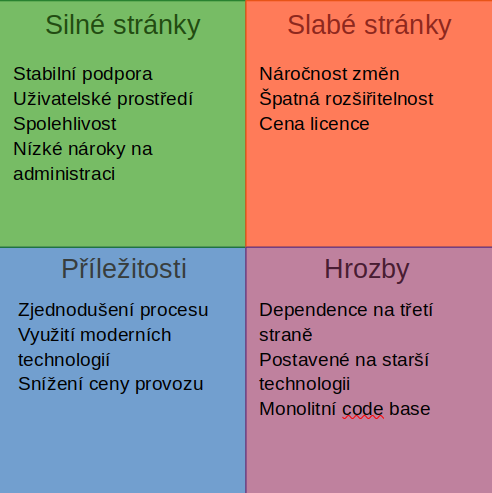
\includegraphics[scale=0.5]{221129-PIS1-SWOT.png}
            \captionof{figure}{SWOT Analýza}
        \end{center}

        \section*{Návrh budoucího stavu}
        \subsection*{Vyjednání nových licencí.}

        Návrh celkového zefektivnění celého procesu zahájím nejpřístupnějším
        bodem, který může dosáhnout okamžitých výsledků při nízké časové
        investici. Tedy vyjednáním lepších podmínek s dodavatel softwaru. v
        současné době tento dodavatel nabízí různé stupně funkcionalit při
        rozdílných cenách. V tomto konkrétním případě je možné vyjednat
        aktualizaci licencí takovým způsobem, který bude efektivně pokrývat
        všechny potřeby systému bez dalších vedlejších nákladů. Například při
        vývoji vlastního frontendového portálu pro uživatele. Při vyjednávacích
        schůzkách má firma silnou pozici, protože je pro dodavatele významným
        zákazníkem a roční částky za licence se pohybují v horních hranicích
        stovek tisíců dolarů. Další stránkou zefektivnění  tohoto komerčního 
        vztahu může být i dohoda o poskytování služeb podpory. Nastavení
        poskytované podpory je nyní nastaveno na tu nejvyšší možnou úroveň.
        Nicméně je možné v rámci nového modelu dohodnout nižší úroveň bez hrozby
        degradace poskytovaných služeb. Celkově tedy v tomto bodě můžeme poměrně
        rychle a levně dosáhnout výrazné úspory celkových nákladů.

        \subsection*{Přesunutí většiny procesů do cloudového prostředí.}
        Moderní technologie nyní dovolují granulárně nastavit spotřebu
        informačních prostředků k dosažení podnikatelských cílů. Cloudové
        prostředí hraje v tomto návrhu zlepšení procesu důležitou roli. Většina
        současného kódu je nyní nasazena na serverech, které si firma spravuje
        sama. Tím, že části tohoto kódu přesuneme do cloudu, umožníme tím
        konfiguraci dostatečnou granularitu a tím snížit náklady na provoz
        hardwaru i softwaru. Pro tyto účely využijeme cloud Microsoft Azure.
        důvodem je fakt, že celý systém již pracuje s  technologiemi od
        Microsoftu a tudíž bude implementace i správa podstatně jednodušší.
        Nebude také vyžadovat větší míru školení pro administrátory, kteří již
        mají profesionální úroveň znalostí ze své práce s Office 365. Celkově
        tedy změníme backend celého systému, který nebude mít dopad na
        uživatelskou přístupnost.
        
        \subsection*{Automatizace schvalovacího procesu}
        Jeden z hlavních nedostatků je nynějšího řešení jsou dlouhé lhůty ve
        schvalovacím procesu. Protože bude celé řešení situované v cloudu, můžeme
        nadefinovat pracovní postupy, které budou automaticky schvalovat
        žádosti, které nijak nevybočují ze standardní konfigurace pracovních
        prostorů. V takovém případě by uživatel dostal emailovou notifikaci o
        vytvoření pracovního prostor v rámci minut. Žádosti, které by
        vyžadovali specifičtější nastavení by podléhaly speciálnímu ověřovacímu
        automatickému pracovnímu postupu, který by nejprve zkontroloval
        náležitosti a splnění podmínek (jako například splněné školení uživatele)
        a teprve poté by pracovní prostor vytvořil. Opět se v tomto scénáři
        pohybujeme v rámci minut od počátečního zadání požadavku. Pouze v
        případě, že bude zaslaný požadavek velice specifický a bude vyžadovat
        zvláštní konfiguraci, bude ho nutné schválit manuálně jedním z
        administrátorů. Takových případů se však neočekává mnoho a většině
        případů uživatel takový prostor neočekává okamžitě. Díky automatizaci
        těchto schvalovacích procesů, budeme schopni odbavit 95\% všech žádostí
        v rámci minut a pouze zlomek bude vyžadovat větší lidskou pozornost.

        \subsection*{Rozbití monolitního řešení na malé mikroslužby}
        Díky zahrnuté integraci služeb Azure s Office 365 můžeme nadefinovat 
        pracovní postupy jako mikroslužby a tím výrazně snížit celkové zatížení
        systému. Tyto mikroslužby mají vlastní model financování, které je
        většinou navázáno na strojový čas. tedy čas, po který aplikace běží a
        konzumuje výpočetní prostředky. Tento strojový čas je počítán na minuty,
        kde má každá cloudová služba jinou sazbu. Náš systém bude využívat pouze
        základní nabídku služeb, kde se sazby na minutu pohybují v rámci centů
        amerického dolaru. Současný kód je řešen monoliticky, tedy všechny
        metody jsou v jedné code base a tím ztěžují přístupnost
        administrátorského týmu. Tyto metody mohou být z tohoto kódu vyňaty a
        implementovány jako samostatné mikroslužby. Pro tento případ využijeme
        cloudovou službu Azure Functions (AF), která poskytuje prostředí pro různé
        programovací a skriptovací jazyky. Každá metoda tedy bude svou vlastní
        AF, kterou bude možné volat na základě rozhodovacího stromu v dotazníku
        vyplněným uživatelem při zadávání žádosti na pracovní prostor. 
        
        \subsection*{Minimalizace hrozeb v oblasti starších technologií}
        Ne všechen kód bude možné do cloudu převézt. Jedná se zejména o ty
        části, které jsou napojeny na starší systémy hostované v rámci interní
        sítě a nemohou být bez rozsáhle refaktorizace implementovány nově pomocí
        modernějších vývojových metod. Většina takového kódu je stále napsaná v
        zastaralé, ale stále Microsoftem podporované verzi \textit{.NET Framework}.
        Abychom docílili minimalizace případných výpadků z důvodu ukončení
        podpory, musíme tyto často aktualizovat na co nejnovější verzi .NET
        Frameworku, která má posunutou hranici ukončení podpory. Dále je v
        systému nasazen kód, který komunikuje s frontendovými aplikacemi
        hostovaných na interní síti a verze NodeJS je v tomto případě již těsně
        před ukončením oficiální podpory. Zde je nebezpečí ještě větší, protože
        NodeJS je takzvaný \textit{open source} projekt, kde nemá forma velkého
        dovolání v rámci podpory, nýbrž se může pouze obrátit na komunitní
        portál řešení problémů. V tomto případě bude refaktorizace kódu nutná,
        protože jsou jednotlivé funkcionality nekompatibilní s novějšími verzemi
        NodeJS. Z výše uvedeného vyplývá, že musí provézt upgrade na co nejnovější 
        verze, kde je to možné, abychom se vyvarovali bezpečnostním i funkčním
        problémům. Celá tato sekce se může vzít i jako příležitost k revizi kódu
        a jeho vyladění.

        \section*{Požadavky na systém}
        \subsection*{Shoda s požadavky certifikací}
        Protože bude v průběhu zlepšení systému probíhat refaktorizace většiny
        inženýrských řešení, musí celý kód odpovídat mezinárodním standardům na
        vývoj, nasazení, provozu a ukončení softwarového řešení. Celý životní
        cyklus vývoje musí sledovat a dodržovat rámce definované v jednotlivých
        certifikačních a metodologických ustanoveních.

        \subsection*{Snížení doby od požadavku ke zřízení prostoru}
        Celý schvalovací proces musí splňovat následující set funkcionalit.
        Veškeré požadavky, které se nijak nevymykají standardnímu nastavení
        pracovních prostorů, musejí být schváleny bezodkladně. Standardním
        nastavení je zde myšleno, že uživatel nevyžaduje zvláštní nastavení nad
        rámec výchozí konfigurace pracovních prostorů od Microsoftu a firemní
        nadstavby. Schvalovací systém musí být dostupný i mimo pracovní dobu v
        daném regionu a musí neprodleně notifikovat uživatele o svém stavu
        procesu. Pokud se požadovaná konfigurace bude lišit od standardu, musí
        mít systém přístup do dílčích systému k ověření podmínek žádosti nebo
        musí neprodleně notifikovat administrátory systému a nestandardním
        požadavku. Veškeré tyto aktivity musejí být automatizované a vyžadovat
        vstup lidských zdrojů pouze v nezbytně nutných případech. 
        
        \subsection*{Snížení celkových nákladů}
        Nová implementace systému musí snížit náklady na provoz. Tím je myšleno
        zejména snížení nákladů na hosting a strojový čas. Revize smlouvy o
        poskytování softwarové služby dodavatelem třetí strany musí systém
        docílit snížením pravidelných nákladů na licence a poskytovanou službu
        softwarové podpory.

        \subsection*{Snížení závislostí}
        Refaktorizace kódu musí odstranit nebo minimalizovat závislosti plynoucí
        ze stáří softwaru. Tato aktivita musí také zaručit stabilitu a dostupnost
        nového řešení, která odpovídá standardům moderních softwarových služeb.
        Dále musí snížit závislost na dodavateli softwaru třetí strany vlastními
        podprocesy, které budou vyvíjeny společně s refaktorizací řešení a
        přenosem do cloudového prostředí.

        \subsection*{Snížení "man-days" pro administraci}
        Nové řešení musí snížit množství aktivity vydávanou týmem
        administrátorů, jejichž může být alokován na jiné projekty. Řešení musí
        vykazovat vysokou dostupnost a nenáročnost případných oprav. Musí také
        umožnit administrátorům jednoduchou implementaci opravných balíčků a
        aktualizací vydávaných organizacemi použitého softwaru. 

        \section*{Implementace a omezení}
        \subsection*{Konfigurace nových nastavení v rámci dodávaného softwaru}
        S dodatečnou konfigurací dodávaného softwaru se pojí i jistá omezení,
        která plynou z jeho podstaty. Nicméně nám software dovolí nastavit
        znění emailových notifikací, jejich styly a aplikaci firemního
        brandingu. Dále povoluje editaci takzvaných "politik", podle kterých
        bude následně systém postupovat v rámci rozhodovacího stromu. Politikou
        zde chápeme set nastavení a omezení pro jednotlivé pracovní prostory.
        
        Pro přehlednou administraci řešení bude administrátorům k dispozici
        portál, který bude vytvořen pomoci Microsoft PowerBI. Tento nástroj jsem
        vybral hlavně proto, že umožňuje vytvářet frontendové řešení, které
        nevyžaduje hluboké znalosti v programování a mohou si ho tak daní
        administrátoři rozvíjet a spravovat sami. Protože je tento produkt opět
        od společnosti Microsoft, je možné v něm definovat propojení s různými
        službami ať už v rámci Office 365, či Azure cloud službami.
        Administrátoři tak získají takřka instantní přehled o celém SharePoint a
        Teams prostředí s tím, že je možné do budoucna celý portál rozšířit o
        ostatní služby Microsoft Office.

        \subsection*{Vytvoření zázemí pro bezobslužné nasazení (Git, AzureDevOps)}
        Pro co nejvíce možnou kontrolu nad jednotlivými nasazenými verzemi
        musíme nejprve vytvořit prostředí, které bude splňovat veškeré
        inženýrské i administrativní nároky. Pro účelu toho řešení využijeme
        AzureDevOps (ADO) se systémem kontroly verzí zdrojového kódu Git.
        Software ADO umožňuje vývojářům uchovávat kód na jednom místě a díky
        integrované technologii GIT je také dosaženo kontroly nad jeho
        jednotlivými verzemi. Pomocí integrovaných postupů na automatickou
        kompilaci kódu a jeho následnému nasazení zajistíme firmě
        auditovatelnost na té nejnižší úrovni řešení. Protože jeden z požadavků
        mezinárodních standardů je používat v rámci vývoje softwaru různá
        integrační prostředí (DEV, UAT, PRD), můžeme si v rámci systému GIT
        nadefinovat různé postupy, jak tento bod splnit. Pro mé řešení využiji
        možnosti vytváření vývojových větví, které se po úspěšném otestování v
        jednotlivých vývojových prostředích budou přes schvalovací proces a
        kontrole kódu integrovat do hlavní větve zdrojového kódu. ADO také
        dovoluje psát technickou dokumentaci pomocí Markdown syntaxe, a poté
        celý repositář publikovat jako „wiki“ stránky, kde je vše automaticky
        přeloženo do stylů a formátování grafického dokumentu. Tvorba a uchování
        dokumentace je však mimo rozsah této práce, a tudíž ji zde pouze
        zmiňuji. Nemalou součástí celého řešení je také konfigurace CI/CD
        (continuous integration/continuous deployment) pipeline (postupy). Ty
        umožňují automaticky testovat integritu zdrojového kódu a pomáhají v něm
        odchytit chyby již v rané fázi vývoje. Protože jsou agnostické vůči
        programovacím jazykům a vývojovým prostředím, můžeme je využít i k
        nasazení zkompilovaného řešení přímo do Azure cloudových služeb [7].
        Tyto pipelines nakonfiguruji také pro jednotlivá vývojová prostředí pro
        větší kontrolu nad vývojem. Celý proces vývoje a testování kódu bude
        tedy zcela automatizované.

        \subsection*{Nasazení a konfigurace služeb}
        Konfigurace infrastruktury je v tomto ohledu neméně důležitá. Celé
        řešení bude využívat princip CaaC neboli Configuration as a Code
        (Konfigurace přes zdrojový kód). Protože Microsoft Azure poskytuje
        technologii ARM šablon, celá infrastruktura může být nasazena
        automaticky, a dokonce s identickou konfigurací pro jednotlivá vývojová
        prostředí. Opět zde využijeme Azure DevOps s jeho integrovanými postupy
        pro nasazení řešení. Konkrétně v tomto případě využiji již zmínění
        PowerShell. Protože má Microsoft detailně zdokumentované potupy, jak ARM
        šablony vytvářet a používat, je tento směr nejméně zatěžující v rámci
        údržby několika vývojových prostředí. Navíc můžeme ARM šablony
        automaticky vygenerovat přímo v Azure portále a poté je pouze lehce
        upravit, aby splňovaly naše potřeby.  
        
        Nyní nastíním technologie, které budou zodpovědné za exekuci
        jednotlivých procedur, které budou nepřímo kopírovat požadavky na systém
        jako takový. Začnu  prostředím pro jednoduchou správu nad rozhodovacím
        stromem. To znamená kdy a které funkce se budou vykonávat při konkrétním
        scénáři. Zde využijeme Azure Data Factory (ADF). Jedná se o přehledné
        grafické prostředí, které uživateli dovoluje vizuálně nakonfigurovat
        postup (pipeline) akcí, které se v dané rozhodovací větvi vykoná. ADF je
        veden jako nástroj pro zpracování „Big data“, a má tudíž zabudovanou
        konektivitu do různých služeb v rámci Azure cloudu. Dovoluje nám také
        přehledně nakonfigurovat síťové prvky, které poté implicitně zvýší
        bezpečnost celého řešení.

        \subsection*{Softwarová omezení}
        Celková softwarová omezení se pevně váží s navrhovanou cloudovou
        infrastrukturou. I když Microsoft přináší stále lepší podmínky pro
        přizpůsobení jednotlivých služeb, stále se administrátoři i vývojáři musí
        potýkat s hranicemi dodávaného softwaru. Velkou úlohu zde hrají i limity
        na API (Application Programming Interface) volání, které jsou sice
        definovány v tisících za minutu, pokud ale spustíme složitější
        automatizaci, může být aplikaci zabráněno v dalším běhu a tudíž by se
        celý systém na určitou dobu zastavil. V tomto případě bychom hovořili o
        degradaci služby a musíme takovou skutečnost promítnout do úprav
        požadavků na systém. Zřídkakdy však k takovým omezení dochází a proto
        můžeme uvézt dostupnost 95\%.

        \subsection*{Omezení z hlediska financí}
        I když je tento návrh koncipován do podoby, který je z hlediska
        implementace proveditelný ve středním časovém horizontu, musíme vzít v
        potaz i uvolněné finance na celý projekt. Nyní nastíním jednotlivá
        odvětví, která budou vyžadovat přímé náklady na projekt. Hlavní
        aktivitou, která bude vyžadovat největší část investice je implementace a
        konfigurace cloudových služeb. Protože se musí monolitní kód
        refaktorovat do menších mikro služeb, vyžádá si tato aktivita nejvíce
        finančních i časových prostředků. Pokud nebude možné financovat celý
        přesun do cloudu, je možné přenést pouze nejnutnější komponenty, které
        jsou zodpovědné za schvalovací proces. Ten je v konečném důsledku
        zodpovědný za majoritu funkcí, jejichž modernizací docílíme nejlepších
        výsledků v efektivitě celého systému.

        Dalším omezením může být i samotné vyjednávání o ceně licencí a úrovní 
        podpory od dodavatele softwaru pro frontendové řešení. Pokud by
        dodavatel nesouhlasil s novými podmínkami, mohlo by dojít v nejhorším
        případě i ke komplikacím v oblasti poptávání nového řešení. Vzhledem k
        časové citlivosti i citlivosti systému by mohly také vzniknout
        nedostatky ve výběrových řízeních a akceptování nového dodavatele s
        horšími podmínkami.  
        
        I když je tým administrátorů zkušený v oblasti technologií od Microsoftu,
        přeci jenom na ně bude kladen důraz na osvojení si způsobu práce s
        cloudovým prostředím. Zde může dojít k omezení z pohledu personální
        kapacity, kdy se může pouze část týmu věnovat adopci nových postupů.

        \section*{Závěr}
        Celý návrh řešení optimalizace systému je koncipován tak, aby byl co
        nejméně invazivní do běžného provozu. Protože firma podniká ve velice
        regulovaném prostředí, musí se řídit metodikami pro nasazování a
        implementaci nových systémů. To obnáší mnoho výzev. Závěr je tedy
        takový, že je možné provézt změny i za produkčního provozu, kde si firma
        nastaví takzvanou "transition period", během které vytvoří nový design
        systému, alokuje zdroje a vytvoří reálný časový plán. Jak je popsáno v
        předchozí kapitole, nemusejí být aplikovány všechny navrhované změny,
        stačí pouze zefektivnit proces schvalování který signifikantně zlepší
        stabilitu, uživatelskou přívětivost a uvolní pracovní kapacity týmu
        administrátorů.

	\end{spacing}
    \end{sloppypar}
\end{document}

